\documentclass{VUMIFPSkursinis}
\usepackage{algorithmicx}
\usepackage{algorithm}
\usepackage{algpseudocode}
\usepackage{amsfonts}
\usepackage{amsmath}
\usepackage{bm}
\usepackage{caption}
\usepackage{color}
\usepackage{float}
\usepackage{graphicx}
\usepackage{listings}
\usepackage{subfig}
\usepackage{wrapfig}
\usepackage{array}
\usepackage{enumitem}

% Remove spaces between items if needed
%\setitemize{noitemsep}
%\setenumerate{noitemsep}

% Allow having thick borders in a table
\makeatletter
\newcommand{\thickhline}{%
    \noalign {\ifnum 0=`}\fi \hrule height 2pt
    \futurelet \reserved@a \@xhline
}
\newcolumntype{"}{@{\vrule width 2pt}}
\makeatother

% Titulinio aprašas
\university{Vilniaus universitetas}
\faculty{Matematikos ir informatikos fakultetas}
\department{Programų sistemų katedra}
\papertype{Reikalavimų specifikacija, analizė ir techninė struktūra}
\title{Knygų keitimosi klubas}
\titleineng{}
\status{2 kurso 5 grupės studentai}
\author{Vidmantas Bakštys}
\secondauthor{Tadas Petrauskas}
\thirdauthor{Tadas Vaitiekūnas} % Pavardes pagal abecele :)
\supervisor{lekt. dr. Vytautas Valaitis}
\date{Vilnius – 2017}

% Nustatymai
% \setmainfont{Palemonas}   % Pakeisti teksto šriftą į Palemonas (turi būti įdiegtas sistemoje)
\bibliography{bibliografija}

\begin{document}
\maketitle

\setcounter{tocdepth}{2}

\pagenumbering{gobble}  % nerodyti puslapio numberio turinyje
\tableofcontents
\pagenumbering{arabic} 

\setcounter{secnumdepth}{0}

\sectionnonum{Anotacija}
Laboratoriniame darbe apibrėžiami reikalavimai sistemai, struktūrinis dalykinės srities modelis (angl. Domain modelling), preliminarios sistemos atliekamos užduotys (angl. Use case modelling) ir atliekama reikalavimų peržiūra. Darbas atliekamas taikant ICONIX procesą.\\
Darbą įgyvendina Programų sistemų 2 kurso 5 grupės studentai Vidmantas Bakštys, Tadas Petrauskas, Tadas Vaitiekūnas.

\sectionnonum{Įvadas}
Šiame dokumente tobulinama programų sistemos "Knygų keitimosi klubas" (toliau - KKK) architektūra, remiantis ICONIX proceso pirmuoju žingsniu

\subsection{Darbo tikslas}
Remiantis ICONIX procesu, patobulinti esamą sistemą, suteikiant papildomo funkcionalumo vartotojui bei pilnai patenkinant užsakovo poreikius

\subsection{Dalykinė sritis}
Literatūros prekyba ir mainai

\subsection{Probleminė sritis}
Sklandus literatūros vienetų pardavimas ir apsikeitimas jais išvengiant apgaulės ir sukčiavimo atvejų

\subsection{Sistemos naudotojai}
Sistema skirta naudoti registruotiems vartotojams bei sistemos svečiams

%Šiame dokumente pateikiama programų sistemos „Automobilių dalių prekybos platforma" (toliau ADPP) architektūra. Ji yra apibrėžiama aprašant sistemą keliais aspektais (pjūviais), naudojant 4+1 pjūvių modelį. Architektūra buvo projektuojama taip, kad būtų įgyvendinami ankščiau pateikti užsakovo poreikiai, bei remiantis dalykinės srities analize. Šis dokumentas yra skirtas programuotojams, kuriantiems šią sistemą, bei būsimos sistemos administratoriams.
%
\setcounter{secnumdepth}{4}

\section{Reikalavimai}
	Šiame skyriuje pateikiami funkciniai bei nefunkciniai reikalavimai sistemai, apibrėžiantys norimą sistemos pokytį.
	Reikalavimai buvo sudaryti remiantis esama sistema ir užsakavo pateiktais pradiniais reikalavimais,
	kurie yra pateikiami šio dokumento priede.
\subsection{Funkciniai reikalavimai}
	\begin{enumerate}[label=\textbf{FR\arabic*}]
		\item Užsiregistravęs vartotojas gali prisijungti:
			\begin{enumerate}[label*=\textbf{.\arabic*}]
				\item Naudodamasis savo vartotojo vardu (arba elektroniniu paštu) ir slaptažodžiu;
				\item Naudodamasis socialinio tinklo paskyra;
			\end{enumerate}
		\item Norimų gauti knygų sąrašas;
			\begin{enumerate}[label*=\textbf{.\arabic*}]
				\item Kiekvienas registruotas vartotojas gali pridėti knygų prie savo sarašo;
				\item Vartotojas gali įkelti knygą į savo sarašą nurodydamas ISBN kodą;
				\item Vartotojas gali ieškoti knygos internete pagal pavadinimą ar autorių ir 
					pasirinkęs ją įkelti į savo sarašą;
				\item Sistema neleidžia įkelti neegzistuojančios knygos į savo sarašą;
				\item Vartotojai gali matyti savo ir kitų vartotojų sąrašus;
				\item Vartotojui pranešti (el. paštu) kada sistemoje atsiranda knyga, esanti jo saraše;
		    \end{enumerate}
		\item Knygos įkėlimas į sistemą;
			\begin{enumerate}[label*=\textbf{.\arabic*}]
				\item Vartotojas gali įkelti knygą įvesdamas knygos ISBN kodą;
				\item Vartotojas gali ieškoti knygos pagal pavadinimą ar autorių ir 
					pasirinkęs ją įkelti;
				\item Sistema leidžia vartotojui įkelti knygą tik jei knyga su tuo ISBN kodu egzistuoja;
				\item Vartotojas gali pridėti komentarą apie savo įkeltą knygą;
				\item Vartotojo pridėtos knygos puslapyje automatiškai pridėti oficialų aprašymą apie knygą;
			\end{enumerate}
		\item Įkeltų knygų paieška;
			\begin{enumerate}[label*=\textbf{.\arabic*}]
				\item Lankytojas gali ieškoti knygos sistemoje pagal ISBN kodą;
				\item Lankytojas gali ieškoti knygos pagal raktinius žodžius;
				\item Jei knygos sistemoje nėra, ieškoti jos internete, radus pasiūlyti pridėti
					prie norimų gauti knygų sarašo;
				\item Knygos gali ieškoti ir neregistruotas lankytojas;
			\end{enumerate}
		\item Vartotojai gali ieškoti kitų vartotojų, matyti jų puslapius ir su jais susisiekti;
		\item Vartotojas gali pasiūlyti savo įkeltą knygą kitam vartotojui;
		\item Vartotojo puslapyje rodyti išsamią statistiką;
			\begin{enumerate}[label*=\textbf{.\arabic*}]
				\item Sėkmingų mainų skaičius;
				\item Įkeltų knygų skaičius; 
				\item Kitų vartotojų įvertinimai;
				\item Ivertinimų vidurkis;
			\end{enumerate}
	\end{enumerate}
\subsection{Nefunkciniai reikalavimai}
	\begin{enumerate}[label=\textbf{NFR\arabic*}]
		\item Tinklapis turi būti pasiekiamas ir patogus naudoti, per mobilųjį įrenginį;
		\item Turi būti užtikrintas duomenų vientisumas duomenų bazėje;
		\item Turi būti užtikrinta galimybė atkurti duomenų bazės duomenis, įvykus sutrikimams;
		\item Turi būti sukurta sistemos administravimo dokumentacija;
	\end{enumerate}

\section{Struktūrinis dalykinės srities modelis}
	Šiame skyriuje pateikiamas struktūrinis nagrinėjamos dalykinės srities modelis. 
	Modelis pateikiamas UML klasių diagramomis kartu su žodynu - sąrašu esybių su jų aprašymais. 
	\subsection{Esybės}
		Dalykinės srities modelis pateikiamas klasių diagrama (žr. 1 pav.). Ši klasių diagrama yra
		preliminari ir neatspindi visų galutinės sistemos klasių.
		\begin{figure}[H]
			\centering
			\includegraphics[scale=0.7]{img/DomainModel.png}
			\caption{Dalykinės srities esybės}
			\label{img:psi2-domain-model}
		\end{figure}

	\subsection{Žodynas}
		Pateikiami sistemos toliau tekste vartojami esybių pavadinimai su aprašymais:
		\begin{enumerate}[label=\textbf{E\arabic*.}]
			\item Vartotojas - Asmuo, užsiregistravęs (turintis paskyrą) sistemoje;
			\item Lankytojas - Asmuo, apsilankęs tinklapyje (nebūtinai vartotojas);
			\item Knyga - literatūros kūrinys, turintis ISBN kodą;
			\item Įkelta knyga - į KKK sistemą ikelta knyga;
			\item Knygų duomenų bazė - Duomenų bazė, prie kurios sistema jungsis ieškodama knygų, tikrindama ISBN kodus. 
				Ši duomenų bazė KKK sistemai nepriklauso, bet su ja bus bendraujama per specifikuota API.
			\item Knygų duomenų bazės atsakymas - klasė represtentuojantį atsakymą gautą iš knygų duomenų bazės,
				su metodais išnagrinėti informacija jame;
			\item Knygų sąrašas - bet kokių knygų rinkinys;
			\item Ikeltų knygų katalogas - sąrašas visų į KKK sistemą įkeltų knygų;
			\item Knygos aprašymas - oficialus knygos aprašymas, paimtas iš knygų duomenų bazės;
			\item Komentaras - Vartotojo komentaras apie savo įkeltą knygą;
			\item Pageidavimų sąrašas - Sarašas knygų, kurias vartotojas norėtų įsigyti;
			\item Vartotojo puslapis - vartotojo turimas paskyros puslapis, kuriame patalpinta visa viešai matoma vartotojo informacija;
			\item Paieškos rezultatas - knygos paieškos knygų duomenų bazėje rezultatas, ar KKK sistemoje rezultatas;
			\item Vartotojo statistika - Statistinė informacija apie vartotojo paskyrą: sėkmingų mainų skaičius, įkeltų knygų skaičius,
				kitų vartotojų įvertinimai, įvertinimų vidurkis;
			\item Įkeltos knygos puslapis - puslapis, kuriame rodoma visas įkeltos knygos informacija, įskaitant ir ikėlėjo komentarą;
			\item Vartotjų sąrašas duomenų bazėje - sąrašas duomenų bazėje užregistruotų ir saugomų vartotojų;
		\end{enumerate}

	\subsection{Reikalavimų - esybių atsekamumo matrica}\label{strukturinisDSModelis_matrica}
		Reikalavimų - esybių atsekamumo matrica (žr. 1 lentelė) yra skirta atsekti kuri esybė vykdo kuriuos reikalavimus.
		Kiekviena esybė turi vykdyti bent po vieną reikalavimą ir kiekvienas reikalavimas turi turėti bent po vieną esybę.
			\begin{table}[H]\footnotesize
  \centering
  \caption{Reikalavimų - esybių atsekamumo matrica}
  \resizebox{\textwidth}{!}
  {\begin{tabular}{|l| l| l| l| l| l| l| l|} \hline
    	X		& FR1		& FR2		& FR3		& FR4		& FR5		& FR6		& FR7\\
\hline
	E1		&+		&+		&+		&+		&+		&+		&+\\
\hline
	E2		&		&		&		&+		&		&		&\\
\hline
	E3		&		&+		&+		&+		&		&		&+\\
\hline
	E4		&		&+		&+		&+		&		&+		&+\\
\hline
	E5		&		&+		&+		&+		&		&		&\\
\hline
	E6		&		&+		&+		&+		&		&		&+\\
\hline
	E7		&		&+		&+		&+		&		&		&\\
\hline
	E8		&		&		&+		&+		&		&		&\\
\hline
	E9		&		&		&+		&		&		&		&+\\
\hline
	E10		&		&		&+		&+		&		&		&\\
\hline
	E11		&		&		&+		&		&+		&+		&+\\
\hline
	E12		&		&		&+		&+		&		&		&\\
\hline
	E13		&		&		&		&		&+		&		&+\\
\hline
	E14		&		&		&		&		&		&+		&\\
\hline
  \end{tabular}}
  \label{tab:table example}
\end{table}

\section{Užduotys}
	Šiame skyriuje pateikiamos sistemos atliekamos užduotys, 
	jų pagrindiniai bei alternatyvūs scenarijai.
	\begin{figure}[H]
		\centering
		\includegraphics[scale=0.62]{img/UseCase.png}
		\caption{Užduočių diagrama}
		\label{img:psi2-use-case}
	\end{figure}
	\subsection{Užduočių aprašymai}
		Toliau pateikiami visų funkcinius reikalavimus vykdančių užduočių aprašymai. 
		Aprašymų tikslas - aprašyti ką sistema turi daryti vartotojui norint įvykdyti vieną ar kitą užduotį,
		todėl jie yra pateikiami vartotojo užklausos - sistemos atsakymo forma.
		Taip pat šalia kiekvienos užduotys yra pateikiamos sekų diagramos,
		detaliai pavaizduojančios užduoties vykdyma, esybių sąveiką ir priskiriančios
		operacijas klasėms.
		\begin{enumerate}[label=\textbf{U\arabic*.}]
			%TODO: gui eskizai
			\item \textbf{Užsiregistruoti};		
				Lankytojas, būdamas pagrindiniame puslapyje, paspaudžia mygtuką „užsiregistruoti.“ Sistema parodo registracijos langą, kuriame yra registracijos forma.
				Lankytojas suveda savo pasirinktą vartotojo vardą, elektroninį paštą bei slaptažodį, taip pat, jei nori, 
				papildomą informaciją: gyvenamąją vietą, amžių. Tada lankytojas paspaudžia „patvirtinti.“ 
				Sistema patikrina, ar įvesta informacija yra tinkama, sukuria naują vartotojo paskyrą ir prideda ją prie vartotojų sąrašo duomenų bazėje.
				Sistema išsiunčia patvirtinimo laišką nurodytu el. paštu. 
				Lankytojas patvirtina savo registraciją paspausdamas nuorodą gautame laiške. Sistema, gavusi patvirtinimą, išsaugo vartotoją duomenų bazėje kaip patvirtintą,
				pakeičia lankytojo statusą į prisijungusį bei parodo pagrindinį tinklapio puslapį.\\
				\textbf{Alternatyvūs scenarijai:}
				\begin{itemize}
					\item Jei lankytojo suvesta informacija nėra tinkama, sistema parodo pranešimą apie tai, nurodydama kurios įvestys nėra tinkamos.
					\item Jei vartotojo paskyra nėra patvirtinama per 24 valandas, sistema panaikina vartotojo paskyrą duomenų bazėje.
					\item Jei lankytojas registracijos formoje paspaudžia mygtuką „tęsti su facebook“, sistema inicijuoja registraciją per soc. tinklą.
	                    Naršyklė lankytojo paprašo patvirtinti, kad leidžia perduoti facebook vartotojo duomenis sistemai.
						Sistema gauna pagrindinę vartotojo informacija iš "Facebook" bei sukuria naują vartotojo paskyrą duomenų bazėje.
						Sistema pakeičia lankytojo statusą į prisijungusį bei parodo pagrindinį puslapį.
						\begin{itemize}
							\item Jei lankytojas nėra prisijungęs prie "Facebook" naršyklėje, jis nukreipiamas į "Facebook" prisijungimo langą. 
								Lankytojas prisijungia, tuomet sistema tęsia registracijos procesą.
							\item Jei įvyksta sutrikimai asocijuojant lankytoją su "Facebook" paskyra arba lankytojas atsisako patvirtinti informacijos perdavimą,
								sistema vartotoją gražina į registracijos puslapį.
						\end{itemize}
				\end{itemize}
			\item \textbf{Prisijungti;}
				Būdamas pagrindiniame puslapyje, lankytojas įveda savo vartotojo vardą (ar elektroninį paštą) ir slaptažodį į tam skirtus laukelius bei spaudžia prisijungti.
				Sistema patikrina, ar vartotojas su tokiu prisijungimo vardu arba el. paštu yra vartotojų sąraše duomenų bazėje.
				Tada sistema patikrina, ar įvestas slaptažodis yra vartotojo. Sistema pakeičia lankytojo statusą į prisijungusį ir parodo pagrindinį puslapį.\\
				\textbf{Alternatyvūs scenarijai:}
				\begin{itemize}
					\item Jei vartotojas su tokiais duomenimis nerastas, apie tai išsiunčiamas pranešimas;
					\item Jei vartotojo slaptažodis neteisingas, jam parodomas pranešimas apie tai ir leidžiama bandyti dar kartą;
					\item Jei lankytojas paspaudžia mygtuką „prisijungti su facebook“, sistema inicijuoja prisijungimą per "Facebook";
						\begin{itemize}
							\item Jei lankytojas nėra prisijungęs prie "Facebook" naršyklėje, jis nukreipiamas į "Facebook" prisijungimo langą. 
								Lankytojas prisijungia, tuomet sistema tęsia prisijungimo procesą;
							\item Jei įvyksta sutrikimai asocijuojant lankytoją su "Facebook" paskyra arba lankytojas atsisako patvirtinti informacijos perdavimą,
								sistema vartotoją gražina į pagrindinį puslapį;
							\item Jei lankytojo "Facebook" paskyra nėra asocijuota su jokiu KKK sistemos vartotoju, sistema inicijuoja vartotojo registraciją per "Facebook" (žr. U1: alternatyvūs scenarijai);
						\end{itemize}
				\end{itemize}
			\item \textbf{Pridėti knygą prie pageidavimų sąrašo;} \\
				Vartotojas, būdamas pagrindiniame puslapyje, paspaudžia mygtuką „pridėti knygą prie pageidavimų sąrašo“. 
				Sistema vykdo užduotį „Ieškoti knygos knygų duomenų bazėje“ (žr. U6).
				Vartotojas rastų knygų saraše pasirenka vieną iš knygų ir paspaudžia mygtuką „pridėti pasirinktą knygą“.
				Sistema vykdo užduotį „pridėti pasirinktą knygą prie pageidavimų sąrašo“ (žr. U7).
				\begin{figure}[H]
					\centering
					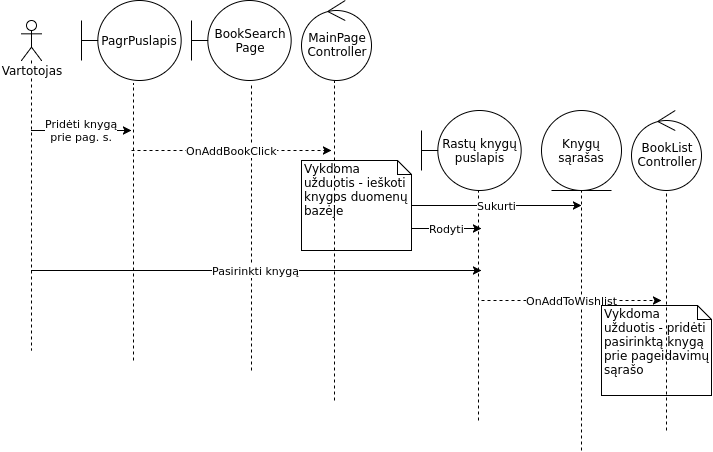
\includegraphics[scale=0.7]{img/U3-sequence.png}
					\caption{U3 sekų diagrama}
					\label{img:psi2-u3-sequence}
				\end{figure}
			\item \textbf{Įkelti knygą į sistemą;}\\
				Vartotojas, būdamas pagrindiniame puslapyje, paspaudžia mygtuką „Įkelti knygą“. Sistema vykdo užduotį „Ieškoti knygos knygų duomenų bazėje“ (žr. U6).
				Vartotojas rastų knygų saraše pasirenka vieną iš knygų. Sistema iš knygų sąrašo paima pasirinktą knygą ir paima jos aprašymą.
				Sistema parodo knygos pridėjimo langą, kurį užpildo informacija apie knygą (autorius, pavadinimas, leidimo metai, aprašymas). Vartotojas prideda savo komentarus apie knygą ir apie
				savo turimą egzempliorių. Vartotojas paspaudžia mygtuką „išsaugoti“. Sistema patikrina, ar vartotojo įvestas komentaras nėra per ilgas.
				Sistema išsaugo knygą ir visą jos informaciją įkeltų knygų kataloge. Vartotojui parodomas pranešimas, kad knyga sėkmingai įkelta.\\
				\textbf{Alternatyvūs scenarijai:}
				\begin{itemize}
					\item Jei sistemai nepavyksta susisiekti su knygų duomenų baze arba negaunamas atsakymas su knygos aprašymu, vartotojui parodomas pranešimas apie sutrikimą.
					\item Jei vartotojo pridėtas komentaras yra per ilgas, vartotojui parodomas pranešimas apie tai.
					\item Jei dėl kokių nors priežasčių knygos nepavyko išsaugoti įkeltų knygų saraše, vartotojui parodomas pranešimas ir paprašoma bandyti vėliau.
				\end{itemize}
				\begin{figure}[H]
					\centering
					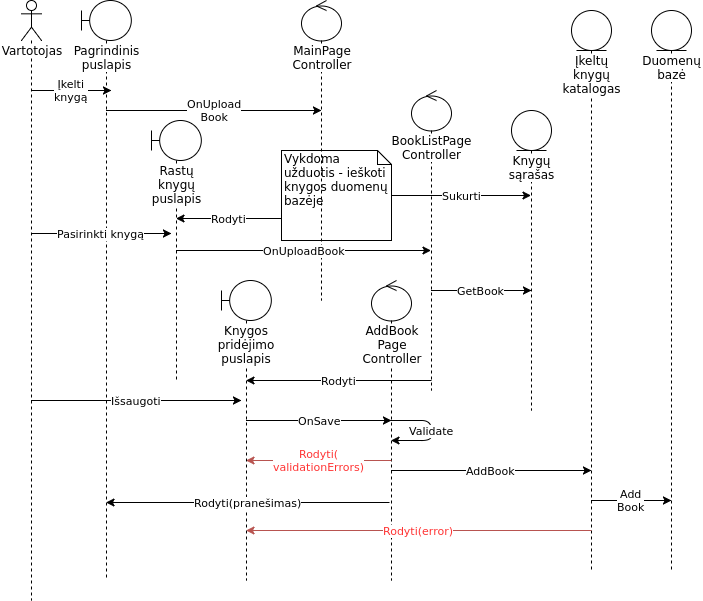
\includegraphics[scale=0.7]{img/U4-sequence.png}
					\caption{U4 sekų diagrama}
					\label{img:psi2-u4-sequence}
				\end{figure}
			\item \textbf{Ieškoti knygos įkeltų knygų kataloge;}\\
				Lankytojas, būdamas pagrindiniame puslapyje, paspaudžia mygtuką „Ieškoti knygos.“ Sistema parodo knygos ieškojimo langą.
				Lankytojas pasirenka, ar ieškoti pagal ISBN kodą, ar pagal raktinius žodžius. 
				Lankytojas įveda ISBN kodą arba raktažodžius ir paspaudžia „ieškoti.“ Sistema patikrina, ar įvestis yra validi.
				Sistema pagal vartotojo įvestį ieško knygos įkeltų knygų kataloge. 
				Jei buvo rasta bent viena knyga, sistema parodo rastų knygų sąrašą vartotojui. Vartotojas pasirenka vieną iš rastų knygų.
				Sistema parodo įkeltos knygos puslapį (žr. U8).\\
				\textbf{Alternatyvūs scenarijai:}
				\begin{itemize}
					\item Jei lankytojo įvestis nėra validi, sistema parodo pranešimą. Lankytojas įveda ISBN kodą arba raktažodžius iš naujo.
					\item Jei knyga nebuvo rasta įkeltų knygų kataloge, sistema parodo pranešimą, kad įkeltų knygų kataloge knyga nerasta 
						ir atlieka paiešką knygų duomenų bazėje, naudodama tą pačią vartotojo įvestį (žr. U6). Jei paieška buvo sėkminga ir buvo rasta bent viena knyga, 
						sistema rezultatų lange parodo rastų knygų sąrašą. Lankytojas pasirenka knygą iš rastų knygų sąrašo.
						Sistema parodo informaciją apie knygą, jos aprašymą. Jei lankytojas yra vartotojas, jis gali paspausti mygtuką „pridėti pasirinktą knygą prie pageidavimų sąrašo“ (žr. U7).
						Kitu atveju jam pasiūloma užsiregistruoti (žr. U1).
				\end{itemize}
				\begin{figure}[H]
					\centering
					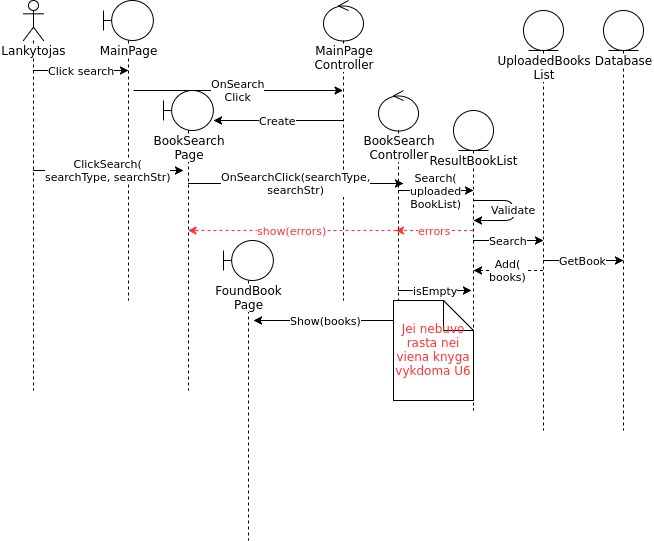
\includegraphics[scale=0.7]{img/U5-sequence.png}
					\caption{U5 sekų diagrama}
					\label{img:psi2-u5-sequence}
				\end{figure}
			\item \textbf{Ieškoti knygos knygų duomenų bazėje}\\
				Sistema, vykdydama kitas užduotis, gauna komandą ieškoti knygos išorinėje knygų duomenų bazėje. 
				Sistema lankytojui parodo knygos paieškos langą. Lankytojas pasirenka, ar nori knygos ieškoti pagal
				ISBN kodą, ar pagal raktažodžius (autorių ar pavadinimą) ir paspaudžia ieškoti. Lankytojas įveda ISBN kodą arba raktažodžius.
				Sistema patikrina, ar įvestis yra validi. Sistema, naudodama lankytojo įvestį, sukuria užklausą knygų duomenų bazei. 
				Sistema gauna atsakymą ir patikrina, ar buvo gauta bent viena knyga. Sistema parodo rastų knygų sąrašą.\\
				\textbf{Alternatyvūs scenarijai:}
				\begin{itemize}
					\item Jei lankytojo įvestas ISBN kodas nėra validus, sistema parodo pranešimą ir laukia naujos įvesties;
					\item Jei dėl kokių nors priežasčių sistemai nepavyksta susisiekti su knygų duomenų baze arba 
						gautas neigiamas atsakymas ar nerasta nei viena knyga, lankytojui parodomas pranešimas apie tai;
					\item Jei knygų duomenų bazė neranda nei vienos knygos, naudodama lankytojo įvestį, vartotojui apie tai pranešama. 
						Lankytojas gali pakeisti įvestį ir ieškoti iš naujo;
				\end{itemize}
				\begin{figure}[H]
					\centering
					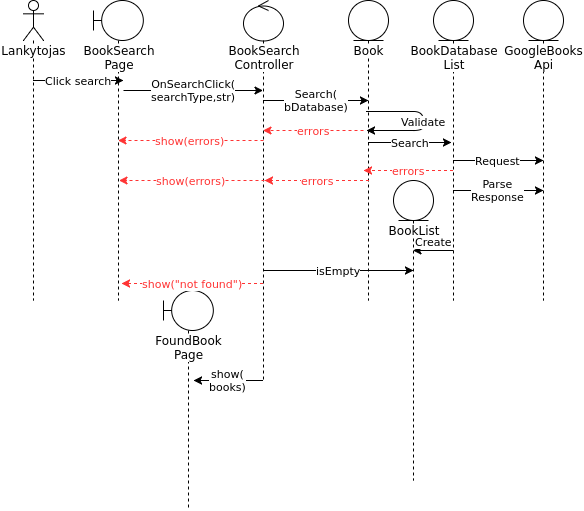
\includegraphics[scale=0.7]{img/U6-sequence.png}
					\caption{U6 sekų diagrama}
					\label{img:psi2-u6-sequence}
				\end{figure}
			\item \textbf{Pridėti pasirinktą knygą prie pageidavimų sąrašo}\\
				Sistema, vykdydama kitas užduotis, gauna komandą pridėti pasirinktą knygą prie pageidavimų sąrašo.
				Sistema patikrina, ar knygos dar nėra vartotojo pageidavimų sąraše duomenų bazėje, ir knygą prideda.
				Vartotojui parodomas pranešimas, kad knyga sėkmingai pridėta.\\
				\textbf{Alternatyvūs scenarijai:}
				\begin{itemize}
					\item Jei vartotojo pasirinkta knyga jau yra jo pageidavimų sąraše, vartotojui apie tai pranešama. Knyga nėra pridedama prie pageidavimų sąrašo;
				\end{itemize}
				\begin{figure}[H]
					\centering
					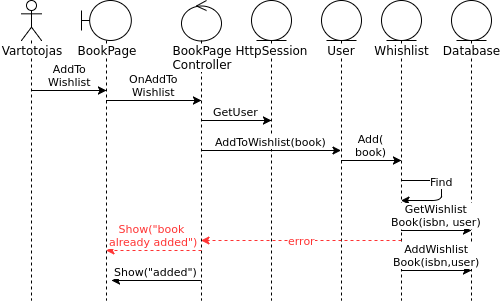
\includegraphics[scale=0.7]{img/U7-sequence.png}
					\caption{U7 sekų diagrama}
					\label{img:psi2-u7-sequence}
				\end{figure}
			\item \textbf{Peržiūreti vartotojo puslapį;}\\
				Vartotojas paspaudžia paryškintą kito vartotojo vardą prie skelbimo ir yra nukreipiamas į pasirinktojo vartotojo puslapį, kuriame mato pasirinktojo vartotojo statistiką, siūlomas knygas bei komentarus. 
				Vartotojo puslapyje kitas vartotojas, paspaudęs mygtuką „siūlyti knygą“, gali pirmajam vartotojui pasiūlyti pirkti knygą iš savo parduodamų knygų sąrašo.
				Vartotojo puslapyje kitam vartotojui, paspaudusiam mygtuką „siųsti laišką", atsiveria langas su „Pavadinimo"" ir „Teksto“ laukais. Užpildęs laukus, vartotojas gali išsiųsti vartotojo puslapio savininkui laišką. 
				Vartotojo puslapyje vartotojas gali įvertinti vartotoją - puslapio savininką kaip knygos pardavėją reitingu žvaigždutėmis (nuo 1 iki 5).
				Vartotojas - puslapio savininkas negali ištrinti kitų vartotojų įvertinimų, jų vidurkis pateikiamas viešai vartotojo puslapyje.\\
				\textbf{Alternatyvūs scenarijai:}
				\begin{itemize}
					\item Vartotojas naudojasi sistemos vartotojų paieška, kurioje įveda paieškos frazę. Sistema pagal frazę, kaip paieškos raktą, parodo vartotojui vartotojų sąrašą.  Vartotojas pasirenka norimą vartotojo vardą ir paspaudęs ant jo yra nukreipiamas į pasirinktojo vartotojo puslapį.
					\item Jei vartotojo puslapis nepasiekiamas, nebeegzistuoja ar įvyko sistemos klaida, vartotojui apie tai pranešama ir jis lieka esamame puslapyje.
					\item Jei vartotojas yra savo paties puslapyje, paspaudęs mygtuką "Skaityti laiškus" jis nukreipiamas į savo pašto dėžutę, kurioje mato atsiųstus jam laiškus.
				\end{itemize}
			\item \textbf{Peržiūrėti įkeltos knygos puslapį}\\
				Vartotojui paspaudus paryškintą knygos pavadinimą kito vartotojo knygų sąrašo ar paieškos puslapyje, sistema nukreipia vartotoją į pasirinktosios knygos puslapį.
				Knygos puslapyje vartotojas mato knygos informaciją, isbn kodą, autorių, knygos savininkų paliktus komentarus (apie knygos būklę ir t.t.) bei kitų vartotojų komentarus.
				Vartotojas knygos puslapyje gali palikti savo komentarą, užpildęs „Pavadinimo“ ir „Teksto“ laukus bei paspaudęs mygtuką „Siųsti komentarą“. Vartotojas taip pat gali palikti knygos įvertinimą žvaigždutėmis (nuo 1 iki 5).\\
				\textbf{Alternatyvūs scenarijai:}
				\begin{itemize}
					\item Jei knygos puslapis nepasiekiamas, nebeegzistuoja ar įvyko sistemos klaida, vartotojui apie tai pranešama ir jis lieka esamame puslapyje.
				\end{itemize}

			\item \textbf{Susisiekti su kitais vartotojais;}\\
				Norėdamas susisiekti su kitais vartotojais, vartotojas gali parašyti vartotojui laišką iėjęs į pasirinktojo vartotojo puslapį (žr. U8).\\
				\textbf{Alternatyvūs scenarijai:}
				\begin{itemize}
					\item Vartotojas gali netiesiogiai susisiekti su kitu vartotoju, palikdamas komentarą prie jo knygos ir tikėdamasis, kad kitas vartotojas jam atsakys laišku ar tuose pačiuose komentaruose.
				\end{itemize}
			\item \textbf{Susisiekti su pardavėju;}\\
				Norėdamas susisiekti su knygos pardavėju, vartotojas knygos puslapyje paspaudžia paryškintą vartotojo vardą ir patenka į vartotojo (pardavėjo) puslapį. Vartotojo puslapyje jis gali išsiųsti pardavėjui laišką (žr. U8).\\
				\textbf{Alternatyvūs scenarijai:}
				\begin{itemize}
					\item Vartotojas gali netiesiogiai susisiekti su pardavėju, palikdamas komentarą prie jo knygos ir tikėdamasis, kad kitas vartotojas jam atsakys laišku ar tuose pačiuose komentaruose (žr. U9).
				\end{itemize}
			\item \textbf{Susisiekti su pirkėju;}\\
				Norėdamas susisiekti su knygos pirkėju, vartotojas knygos puslapyje paspaudžia paryškintą vartotojo vardą ir patenka į vartotojo (pirkėjo) puslapį. Vartotojo puslapyje jis gali išsiųsti pirkėjui laišką (žr. U8).\\
				\textbf{Alternatyvūs scenarijai:}
				\begin{itemize}
					\item Vartotojas gali netiesiogiai susisiekti su knygos pirkėju, palikdamas komentarą prie savo parduodamos knygos ir tikėdamasis, kad pirkėjas jam atsakys laišku ar tuose pačiuose komentaruose (žr. U9).
				\end{itemize}
			\item \textbf{Įvertinti mainus;}\\ % fiksuoti statistiką
				Vartotojas gali įvertinti mainus priskirdamas pardavėjui reitingą (žr. U8) bei reitingą knygai (žr. U9).\\
				\textbf{Alternatyvūs scenarijai:}
				\begin{itemize}
					\item Vartotojas gali parašyti komentarą knygos puslapyje ar vartotojo (pardavėjo) puslapyje.
				\end{itemize}
			\item \textbf{Pasiūlyti savo įkeltą knygą kitam vartotojui;}
				Vartotojas gali pasiūlyti knygą kitam vartotojui šio vartotojo puslapyje paspaudęs mygtuką „Siūlyti knygą“(žr. U8).\\
				\textbf{Alternatyvūs scenarijai:}
				\begin{itemize}
					\item Vartotojas gali kreiptis į kitą vartotoją laišku šio vartotojo puslapyje (žr. U8).
					\item Vartotojas savo nuožiūra gali siūlyti savo knygas kitų knygų puslapiuose, jei mano, kad jo knyga yra susijusi ir gali sudominti pirkėjus.
				\end{itemize}
		\end{enumerate}
	\subsection{Robastiškumo analizė}
		Robastiškumo analizės tikslas - susieti užduotis su objektais (esybėmis), sistemos funkcijomis ir 
		interfeiso elementais. Taip pat yra patikrinamas ir jei reikia pataisomas užduočių tekstas ir statinis sistemos modelis.
		Toliau pateikiamos robastiškumo diagramos kiekvienai užduočiai.
		\begin{enumerate}[label=\textbf{U\arabic*.}]
			\item \textbf{Užsiregistruoti};		
				\begin{figure}[H]
					\centering
					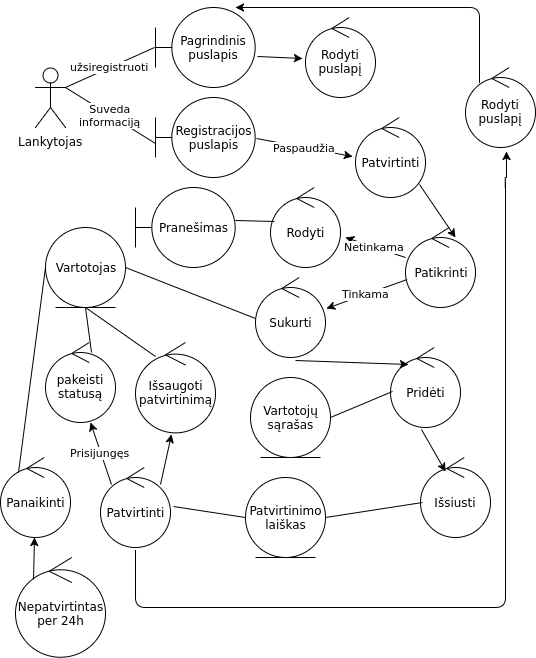
\includegraphics[scale=0.9]{img/U1.png}
					\caption{U1 robastiškumo diagrama}
					\label{img:psi2-u1-robustness}
				\end{figure}
			\item \textbf{Prisijungti;}
				\begin{figure}[H]
					\centering
					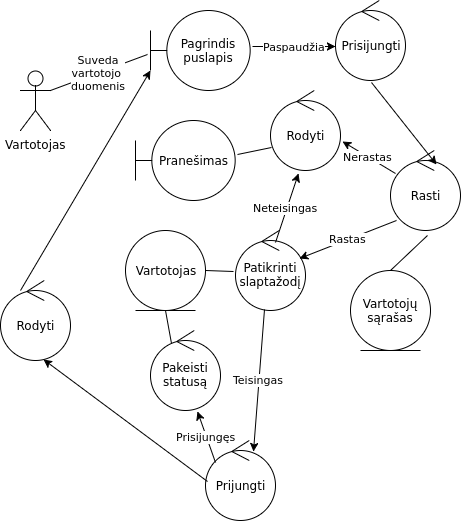
\includegraphics[scale=0.9]{img/U2.png}
					\caption{U2 robastiškumo diagrama}
					\label{img:psi2-u2-robustness}
				\end{figure}
			\item \textbf{Pridėti knygą prie pageidavimų sąrašo;}
				\begin{figure}[H]
					\centering
					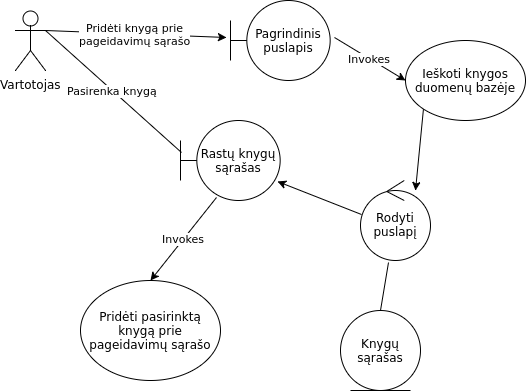
\includegraphics[scale=0.9]{img/U3.png}
					\caption{U3 robastiškumo diagrama}
					\label{img:psi2-u3-robustness}
				\end{figure}
			\item \textbf{Įkelti knygą į sistemą;}
				\begin{figure}[H]
					\centering
					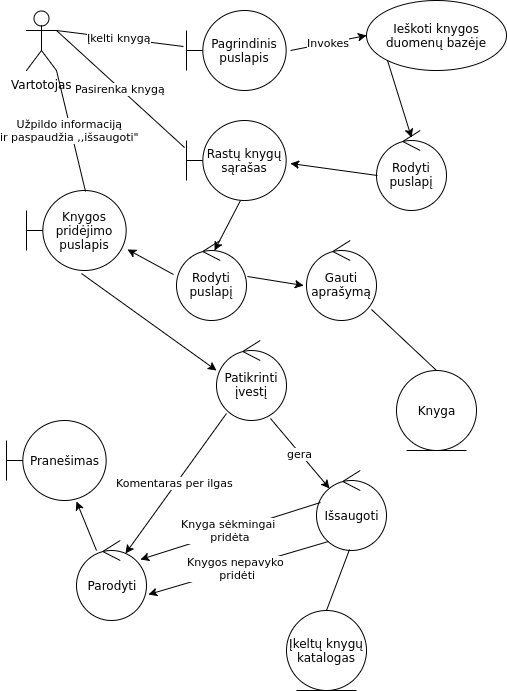
\includegraphics[scale=0.9]{img/U4.png}
					\caption{U4 robastiškumo diagrama}
					\label{img:psi2-u4-robustness}
				\end{figure}
			\item \textbf{Ieškoti knygos įkeltų knygų kataloge;}
				\begin{figure}[H]
					\centering
					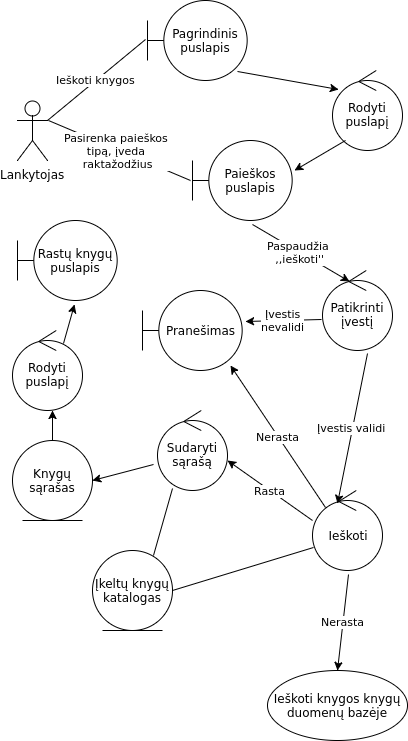
\includegraphics[scale=0.9]{img/U5.png}
					\caption{U5 robastiškumo diagrama}
					\label{img:psi2-u5-robustness}
				\end{figure}
			\item \textbf{Ieškoti knygos knygų duomenų bazėje}
				\begin{figure}[H]
					\centering
					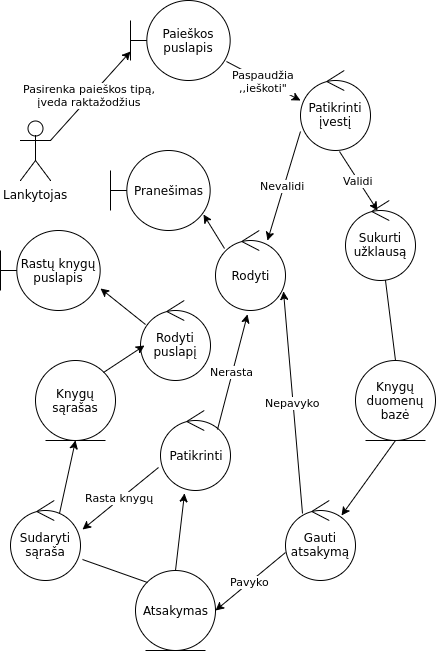
\includegraphics[scale=0.9]{img/U6.png}
					\caption{U6 robastiškumo diagrama}
					\label{img:psi2-u6-robustness}
				\end{figure}
			\item \textbf{Pridėti pasirinktą knygą prie pageidavimų sąrašo}
				\begin{figure}[H]
					\centering
					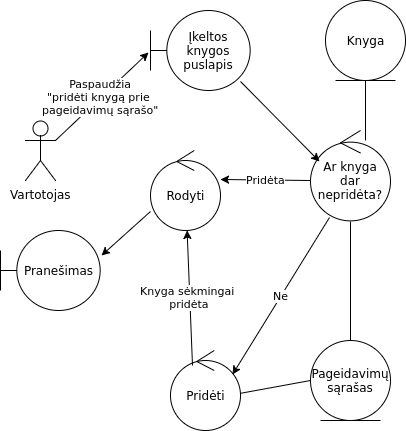
\includegraphics[scale=0.9]{img/U7.png}
					\caption{U7 robastiškumo diagrama}
					\label{img:psi2-u7-robustness}
				\end{figure}
			\item \textbf{Peržiūreti vartotojo puslapį;}
				\begin{figure}[H]
					\centering
					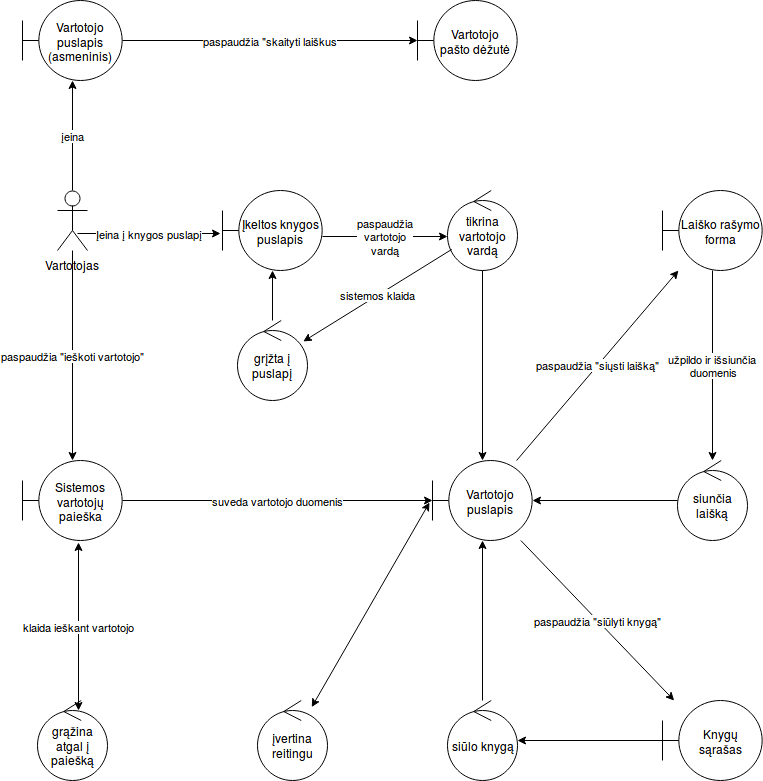
\includegraphics[scale=0.6]{img/U8.png}
					\caption{U8 robastiškumo diagrama}
					\label{img:psi2-u8-robustness}
				\end{figure}
			\item \textbf{Peržiūrėti įkeltos knygos puslapį}
				\begin{figure}[H]
					\centering
					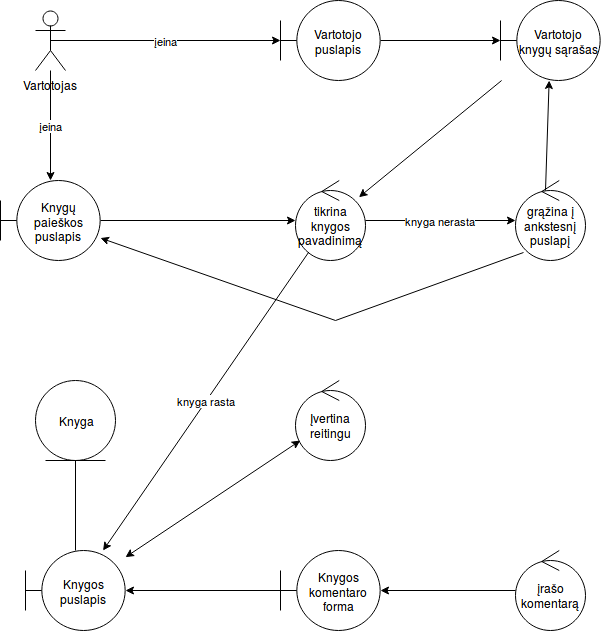
\includegraphics[scale=0.6]{img/U9.png}
					\caption{U9 robastiškumo diagrama}
					\label{img:psi2-u9-robustness}
				\end{figure}
			\item \textbf{Susisiekti su kitais vartotojais;}
				\begin{figure}[H]
					\centering
					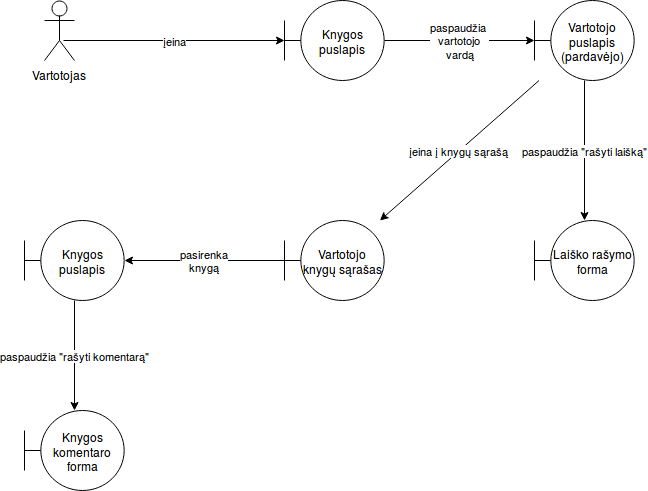
\includegraphics[scale=0.6]{img/U10.png}
					\caption{U10 robastiškumo diagrama}
					\label{img:psi2-u10-robustness}
				\end{figure}
			\item \textbf{Susisiekti su pardavėju;}
				\begin{figure}[H]
					\centering
					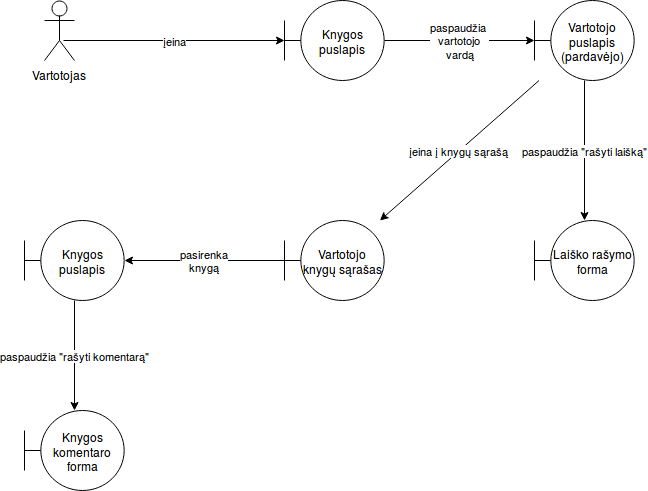
\includegraphics[scale=0.6]{img/U11.png}
					\caption{U11 robastiškumo diagrama}
					\label{img:psi2-u11-robustness}
				\end{figure}
			\item \textbf{Susisiekti su pirkėju;}
				\begin{figure}[H]
					\centering
					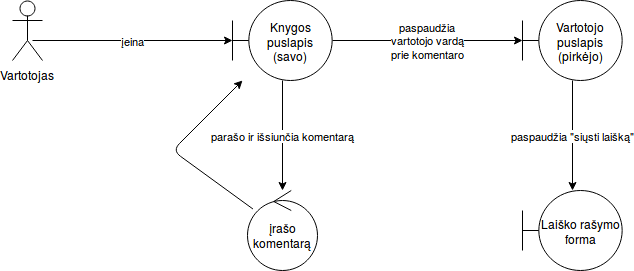
\includegraphics[scale=0.6]{img/U12.png}
					\caption{U12 robastiškumo diagrama}
					\label{img:psi2-u12-robustness}
				\end{figure}
			\item \textbf{Įvertinti mainus;}
				\begin{figure}[H]
					\centering
					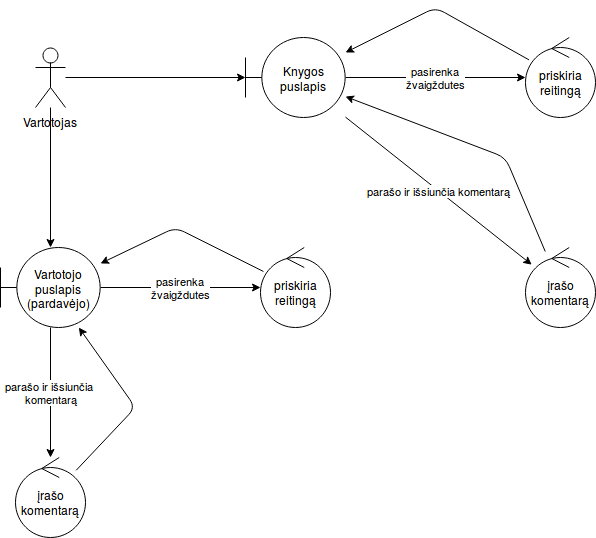
\includegraphics[scale=0.6]{img/U13.png}
					\caption{U13 robastiškumo diagrama}
					\label{img:psi2-u13-robustness}
				\end{figure}
			\item \textbf{Pasiūlyti savo įkeltą knygą kitam vartotojui;}
				\begin{figure}[H]
					\centering
					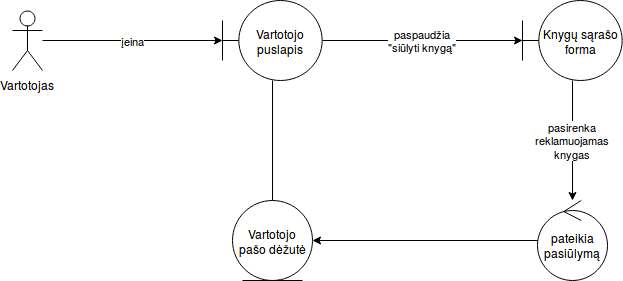
\includegraphics[scale=0.6]{img/U14.png}
					\caption{U14 robastiškumo diagrama}
					\label{img:psi2-u14-robustness}
				\end{figure}
		\end{enumerate}

	\subsection{Reikalavimų - užduočių atsekamumo matrica}\label{strukturinisDSModelis_matrica}
		Reikalavimų - užduočiu atsekamumo matricos (žr 2 lentelė) paskirtis - kiekvianam reikalavimui
		priskirti jį vykdančias užduotis. Kiekviana aprašoma užduotis turi vykdyti kurį nors reikalavimą ir
		kiekvianas reikalavimas turi būti vykdomas bent vienos užduoties.
\begin{table}[H]\footnotesize
  \centering
  \caption{Reikalavimų - užduočių atsekamumo matrica}
  \resizebox{\textwidth}{!}
  {\begin{tabular}{|l| l| l| l| l| l| l| l|} \hline
    	X		& FR1		& FR2		& FR3		& FR4		& FR5		& FR6		& FR7\\
\hline
	U1		&+		&		&		&		&		&		&\\
\hline
	U2		&+		&		&		&		&		&		&\\
\hline
	U3		&		&+		&		&		&		&		&\\
\hline
	U4		&		&+		&+		&+		&		&		&\\
\hline
	U5		&		&+		&		&+		&		&		&\\
\hline
	U6		&		&+		&		&+		&		&		&\\
\hline
	U7		&		&+		&		&		&		&		&\\
\hline
	U8		&		&		&		&		&+		&+		&+\\
\hline
	U9		&		&+		&		&+		&		&+		&\\
\hline
	U10		&		&		&		&		&+		&+		&+\\
\hline
	U11		&		&		&		&		&+		&+		&+\\
\hline
	U12		&		&		&		&		&+		&+		&+\\
\hline
	U13		&		&		&		&		&+		&		&+\\
\hline
	U14		&		&		&		&		&+		&+		&+\\
\hline
  \end{tabular}}
  \label{tab:table example}
\end{table}

\section{Techninė sistemos architektūra}
	Šiame skyriuje pateikiama kuriamos sistemos struktūra, apibrėžiant sistemą sudarančius modulius, jų ryšius, išdėstymą vykdymo aplinkose. 
	\subsection{Sistemos komponentai}
		Sistema yra suskirstyta į vartotojo sąsajos, duomenų ir duomenų saugojimo paketus.
		Komponentams sudaryti buvo naudojamas MVC (model, view, controller) šablonas.
		Vartotojo sąsajos paketą sudaro šie komponentai:
		\begin{itemize}
			\item Puslapių komponentas - yra atsakingas už sąsajos vaizdavimą lankytojui ir atitinka view dalį MVC šablone;
			\item Kontrolerių komponentas - yra tarpininkas tarp vartotojo sąsajos ir duomenų paketo.
				Jis nusprendžia kokius puslapius rodyti ir reaguoja į lankytojo įvestis; 
		\end{itemize}
		Duomenų ir duomenų saugojimo paketai sudaro modelio dalį MVC šablone.
		Komponentai, sudarantys duomenų paketą, yra atsakingi už sistemos logiką.
		Duomenų saugojimo paketą sudaro komponentai, atsakingi už duomenų pakete sukurtų objektų išsaugojimą duomenų bazėje
		bei už prieigą prie išorinės knygų duomenų bazės (naudojant pvz. google books api). 
		Visi komponentai yra vaizduojami komponentų diagramoje (žr. 17 pav.).	
		\begin{figure}[H]
			\centering
			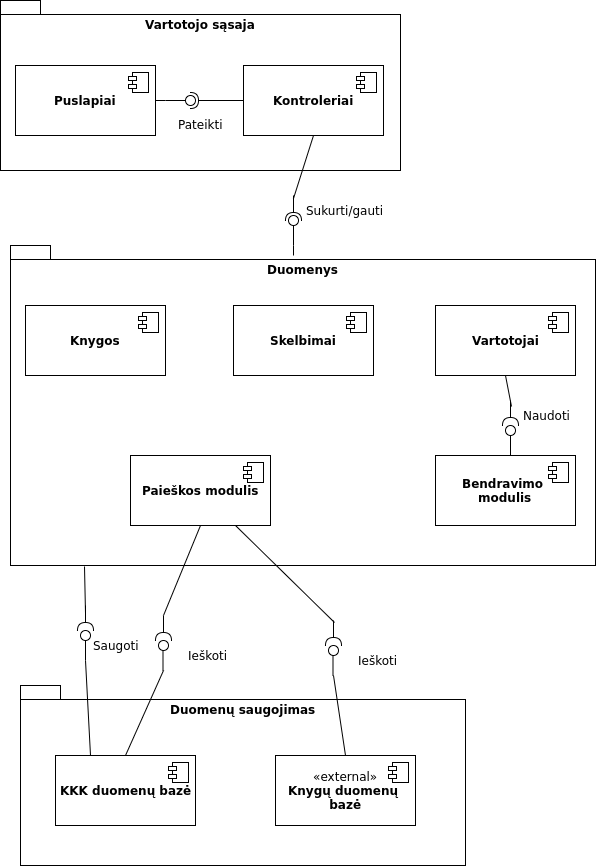
\includegraphics[scale=0.8]{img/Component.png}
			\caption{Komponentų diagrama}
			\label{img:psi2-component}
		\end{figure}
	\subsection{Sistemos komponentų išdėstymas tinkle}
		Sistemos komponentų išdėstymą vykdymo aplinkose vaizduoja diegimo diagrama (žr. 18 pav.).
		Sistemai įgyvendinti reikia web serverio, duomenų bazės bei išorinės (KKK sistemai nepriklausančios) 
		knygų duomenų bazės, kurios prieeinamumas būtų pakankamas.
		Tinklapis turėtų būti prienamas naudojant bet kokią kompiuterio ar mobiliojo įrenginio naršyklę.
		\begin{figure}[H]
			\centering
			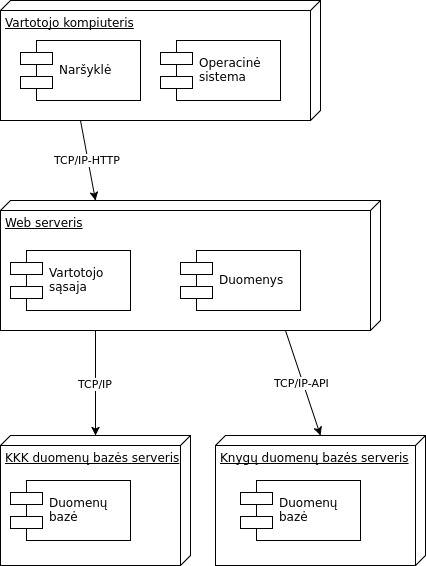
\includegraphics[scale=0.9]{img/Deployment.png}
			\caption{Komponentų išdėstymas tinkle}
			\label{img:psi2-deployment}
		\end{figure}

\section{Testavimo planas ir scenarijai}

\section{Peržiūros metu rastos klaidos}
	Vykdant projektą kiekviename etape yra vykdomos įvairių tipų peržiūros.
	Toliau pateikiamos šių peržiūrų metu rastos klaidos.
	\subsection{Reikalavimų peržiūra}
		Ši peržiūra yra vykdoma apsibrėžus reikalavimus, užduotis, bei stuktūrinį dalykinės srities modelį.
		\begin{itemize}
			\item Gramatinės - sudėti kableliai, pataisyti netaisyklingai parašyti skliaustai;
			\item Rašybos - įrašytos praleistos raidės ir sudėtos nosinės;
		\end{itemize}
	\subsection{Preliminari projekto peržiūra}
		Ši peržiūra yra vykdoma, atlikus robastiškumo analizę.
		\begin{itemize}
			\item Prie kiekvieno skyrelio pridėtas jo aprašymas, paskirtis;
			\item Užduočių tekste nebuvo nurodytas puslapis, iš kurio užduotis prasideda (U3, U4, U5);
			\item Trūkstama knygų duomenų bazės atsakymo klasė statiniame modelyje;
			\item Trūkstama įkeltų knygų katalogo klasė U3 robastiškumo diagramoje;
			\item Trūkstama knygų sąrašo esybė U3 ir U4 robastiškumo diagramose;
			\item Trūkstama knygos esybė U7 robastiškumo diagramoje;
		\end{itemize}
	\subsection{Kritinė projekto peržiūra}
		Ši peržiūra yra vykdoma atlikus sistemos projektavimą,
		t.y. padarius sekų diagramas, ir atnaujinus statinę programų sistemos struktūrą.
		Peržiūros tikslas įsitinti, kad suprojektuota sistema vykdo reikalavimus,
		ir statinis modelis atitinka dinaminį.
		\begin{itemize}
			\item Trūkstami parametrai prie operacijų U3 ir U4 sekų diagramose;
			\item Trūkstama įkeltos knygos klasė ir jos sukūrimo operacija, U4 sekų diagramoje;
			\item Trūkstama įkeltos knygos validacijos operacija U4 diagramoje;
			\item Praleistas knygos radimo, knygų sąraše žingsnis U3 diagramoje;
			\item U5 tekste nepaminėtas mygtuko paspaudimas;
			\item Trūkstama HttpSession klasė statiniame modelyje;
		\end{itemize}
\setcounter{secnumdepth}{0}
\sectionnonum{Priedai}
\subsection{Užsakovo reikalavimai sistemai}
\begin{enumerate}
	\item Leisti vartotojui prisijungti prie sistemos naudojant socialinių tinklų paskyras;
	\item Leisti vartotojui užregistruoti knygą įvedant ISBN kodą;
	\item Kiekvieną kartą vartotojui užregistruojant naują knygą patikrinti pagal ISBN kodą,
		ar knyga egzistuoja. Jei ne, knygos neužregistruoti;
	\item Vartotojui užregistruojant naują knygą, leisti ieškoti knygos pagal 
		nebūtinai pilną pavadinimą arba autorių;
	\item Leisti ieškoti knygos sistemoje pagal ISBN kodą;
	\item Kiekvienam vartotojui leisti susikurti savo norimų gauti knygų sarašą (wishlist);
	\item Neradus ieškomos knygos sistemoje, pasiūlyti ją pridėti prie norimų gauti knygų sarašo;
	\item Suteikti galimybę vartotojui pasiūlyti savo įkeltą knygą kitam vartotojui;
	\item Suteikti galimybę vartotojui ieškoti kitų vartotojų bei susisiekti su jais ne vien
		perkant iš jų knygas;
	\item Vartotojo užregistruotos knygos puslapyje automatiškai pridėti knygos aprašymą
		iš interneto;
	\item Leisti pridėti savo komentarus prie savo įkeltos knygos (apie knygos kokybę,
		pačią knyga ir panašiai);
	\item Vartotojo paskyroje rodyti išsamią vartotojo statistiką (sėkmingų mainų skaičius,
		įvertinimai);
	\item Tinklapis turi būti pasiekiamas ir patogus naudoti per mobilųjį įrenginį;
	\item Turi būti užtikrintas duomenų vientisumas duomenų bazėje;
	\item Turi būti užtikrinta galimybė atkurti duomenų bazės duomenis įvykus sutrikimams;
	\item Turi būti sukurta sistemos administravimo dokumentacija;
\end{enumerate}


\setcounter{secnumdepth}{4}


%FIXME: fix numeration
\sectionnonum{Šaltinių sąrašas}
	\begin{itemize}
		\item http://www.mif.vu.lt/~karolis/PSI2.html
		\item Don Rosenberg, Matt Stephens: Use Case Driven Object Modeling with UML: Theory and Practice, 2007
	\end{itemize}


%\printbibliography[heading=bibintoc]  % Šaltinių sąraše nurodoma panaudota
% literatūra, kitokie šaltiniai. Abėcėlės tvarka išdėstomi darbe panaudotų
% (cituotų, perfrazuotų ar bent paminėtų) mokslo leidinių, kitokių publikacijų
% bibliografiniai aprašai.  Šaltinių sąrašas spausdinamas iš naujo puslapio.
% Aprašai pateikiami netransliteruoti. Šaltinių sąraše negali būti tokių
% šaltinių, kurie nebuvo paminėti tekste.

\end{document}
